\ProjectEntry
{Brain-Inspired Perspective on Configurations: Unsupervised Similarity and Early Cognition}
{First Author}
{Theory, Unsupervised Learning, Brain-Inspired Computation}
{
  \bitem{Studies configurations from a cognitive perspective, relating unsupervised similarity and early cognition.}
  \bitem{Provides theoretical motivation for why configuration structure supports downstream prediction (complementary to GraMixC).}
  \bitem{Connects lineage diagrams, attention structure, and similarity to emergent representation geometry.}
}
{assets/1003_infantconfig/02a_schematic.png}
{\extlink{https://arxiv.org/abs/2510.19229}{arXiv preprint}}
{\badge{Brain-Inspired Computation} \badge{BICS 2025}}

\textbf{Technical Highlights:}
This work formalizes configurations as organizing structures that emerge from unsupervised similarity, offering a brain-inspired account of early category formation. We analyze how a lineage parameter \(\gamma\) controls hierarchical granularity and how energy components (attraction \(h_a\), repulsion \(h_r\)) shape stable configuration landscapes that support downstream learning.

\begin{figure}[ht]
  \centering
  \vspace{-0.5em}
  \subcaptionbox{Lineage (schem.)\label{fig:lineage_schem}}[0.25\linewidth]{%
    \begin{tikzpicture}[
    scale=0.5,
    node distance=8mm and 14mm,
    every node/.style={
        font=\tiny, 
        % minimum width=12mm, minimum height=5mm
    },
    level/.style={rectangle, rounded corners, draw=black, inner sep=2pt},
    ->,>={Stealth[length=2mm]}
]
    \draw[thick,->] (0.5,0) -- (5,0) node[right, font=\tiny] {$\gamma$};
    \draw[thick] (0.5,0.2) -- (0.5,0);
    \draw[thick] (2.75,0.2) -- (2.75,0);
    \draw[thick] (5,0.2) -- (5,0);
    \node[font=\tiny, below] at (0.5,0) {0};
    \node[font=\tiny, below] at (5,0) {$\infty$};
    \node[font=\tiny\bfseries, above] at (0.5,4) {Cfg.0};
    \node[font=\tiny\bfseries, above] at (2.75,4) {Cfg.$n$};
    \node[font=\tiny\bfseries, above] at (4.75,4) {Cfg.$\infty$};
    \node[level, fill=gray!20] (AB) at (0.5,2) {$A \cup B$};
    \node[level, fill=blue!15] (A) at (2.75,3) {$A=\{a_1,a_2\}$};
    \node[level, fill=red!15] (B) at (2.75,1) {$B=\{b_1,b_2\}$};
    \node[level, fill=blue!10] (A1) at (5,3.5) {$a_1$};
    \node[level, fill=blue!10] (A2) at (5,2.5) {$a_2$};
    \node[level, fill=red!10] (B1) at (5,1.5) {$b_1$};
    \node[level, fill=red!10] (B2) at (5,0.5) {$b_2$};
    \draw (AB) -- (A);
    \draw (AB) -- (B);
    \draw (A) -- (A1);
    \draw (A) -- (A2);
    \draw (B) -- (B1);
    \draw (B) -- (B2);
\end{tikzpicture}
%%
  }
  \subcaptionbox{Lineage (CIFAR)\label{fig:lineage_cifar}}[0.2\linewidth]{%
    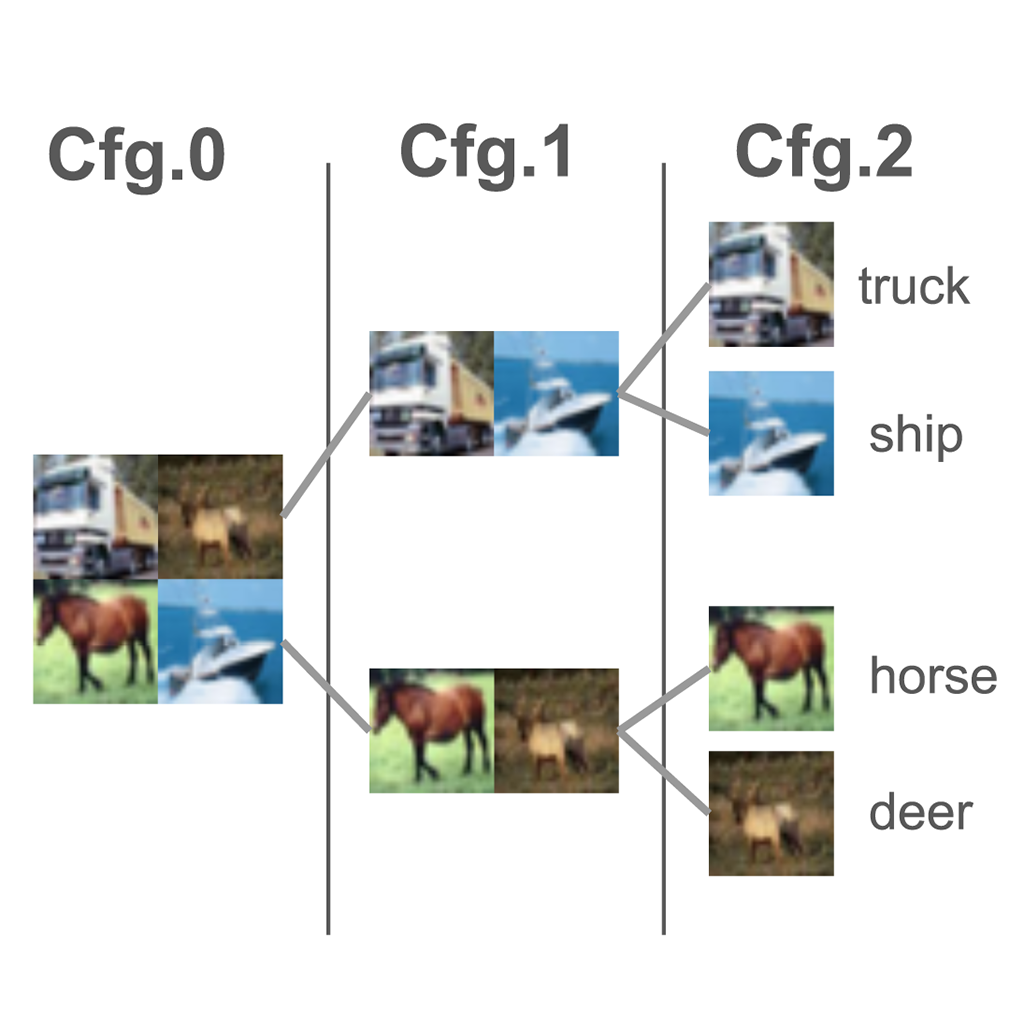
\includegraphics[width=\linewidth]{assets/1003_infantconfig/01_cifar10subset.png}%
  }
  \subcaptionbox{Energy (MNIST)\label{fig:energy_mnist}}[0.237\linewidth]{%
    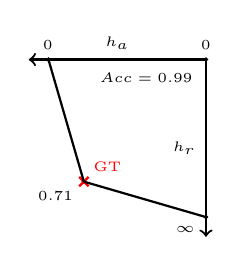
\begin{tikzpicture}[
    scale=0.5,
    every node/.style={
        font=\tiny,
    },
]
    \draw[->,thick] (0,0) -- (-4.5,0) node[midway, above] {$h_a$};
    \draw[->,thick] (0,0) -- (0,-4.5) node[midway, left] {$h_r$};
    \filldraw[black] (0,0) circle (1.2pt);
    \node[anchor=south] at (0,0) {0};
    \filldraw[black] (-4,0) circle (1.2pt);
    \node[anchor=south] at (-4,0) {$\mOmega_{0}$};
    \filldraw[black] (0,-4) circle (1.2pt);
    \node[anchor=north east] at (0,-4) {$\mOmega_{\infty}$};
    \filldraw[black] (-3.1,-3.1) circle (1.2pt);
    \node[anchor=north east] at (-3.1,-3.1) {$\boxed{\mOmega_{0.71}}$};
    \draw[red, thick] (-3.1-0.12, -3.1-0.12) -- (-3.1+0.12, -3.1+0.12);
    \draw[red, thick] (-3.1-0.12, -3.1+0.12) -- (-3.1+0.12, -3.1-0.12);
    \node[anchor=south west] at (-3.1, -3.1) {\color{red}GT};
    \draw[thick] (-4,0) -- (-3.1,-3.1);
    \draw[thick] (-3.1,-3.1) -- (0,-4);
    \node[anchor=north east] at (-0.1, -0.1) {
        $\boxed{\text{Acc}=0.99}$
};
\end{tikzpicture}%
  }
  \subcaptionbox{Energy (WHU)\label{fig:energy_whu}}[0.237\linewidth]{%
    \begin{tikzpicture}[
    scale=0.5,
    every node/.style={
        font=\tiny,
    },
]
    \draw[->,thick] (0,0) -- (-4.5,0) node[midway, above] {$h_a$};
    \draw[->,thick] (0,0) -- (0,-4.5) node[midway, left] {$h_r$};
    \filldraw[black] (0,0) circle (1.2pt);
    \node[anchor=south] at (0,0) {0};
    \filldraw[black] (-4,0) circle (1.2pt);
    \node[anchor=south] at (-4,0) {$\mOmega_{0}$};
    \filldraw[black] (0,-4) circle (1.2pt);
    \node[anchor=north east] at (0,-4) {$\mOmega_{\infty}$};
    \filldraw[black] (-3.5,-2.5) circle (1.2pt);
    \node[anchor=south west] at (-3.5,-2.5) {$\boxed{\mOmega_{0.37}}$};
    \filldraw[black] (-3,-3) circle (1.2pt);
    \node[anchor=north east] at (-3,-3) {$\mOmega_{1.12}$};
    \filldraw[black] (-1.5,-3.8) circle (1.2pt);
    \node[anchor=north east] at (-1.5,-3.8) {$\mOmega_{3.53}$};
    \draw[red, thick] (-3.5-0.12, -2.3-0.12) -- (-3.5+0.12, -2.3+0.12);
    \draw[red, thick] (-3.5-0.12, -2.3+0.12) -- (-3.5+0.12, -2.3-0.12);
    \node[anchor=east] at (-3.5, -2.3) {\color{red}GT};
    \draw[thick] (-4,0) -- (-3.5,-2.5);
    \draw[thick] (-3.5,-2.5) -- (-3,-3);
    \draw[thick] (-3,-3) -- (-1.5,-3.8);
    \draw[thick] (-1.5,-3.8) -- (0,-4);
    \draw[orange,thick, decorate, decoration={brace, amplitude=4pt}]
    ($(-1.45,-3.8)$) -- ($(0,-4)$)
    node[midway, xshift=-0.5mm, yshift=2.5mm]{plateau};
    \node[anchor=north east] at (-0.1, -0.1) {
        $\boxed{\text{Acc}=0.92}$
};
\end{tikzpicture}%
  }
  \caption{
    Configuration lineage and energy landscapes. 
    \textbf{(a)\&(b)} Configuration lineages: $\gamma$ controls hierarchical granularity from coarse to fine. 
    \textbf{(c)\&(d)} Energy landscapes: Axes show attraction $h_a$ and repulsion $h_r$.}
  \label{fig:01_lineage_har}
\end{figure}

\textbf{Key Results:}
\begin{itemize}[leftmargin=1.2em, itemsep=0.1em]
  \item Hierarchical selectivity: superordinate categories stabilize at low \(\gamma\), basic-level categories at higher \(\gamma\), reflecting scale-dependent organization (Fig.~\ref{fig:04_a}).
  \item Novelty detection: energy distributions separate familiar vs. novel inputs (AUC \(\approx\) 0.87), echoing infant habituation paradigms (Fig.~\ref{fig:04_b}).
  \item Dynamic evolution: configurations achieve consistently lower 1/ARI than baselines during category evolution, indicating more stable organization (Fig.~\ref{fig:04_c}).
  \item Geometry: lineage diagrams and energy contours reveal interpretable structure that aligns with emergent representation geometry (Fig.~\ref{fig:01_lineage_har}).
\end{itemize}

\begin{figure}[ht]
  \centering
  \subcaptionbox{Hierarchical Selectivity\label{fig:04_a}}[0.33\linewidth]{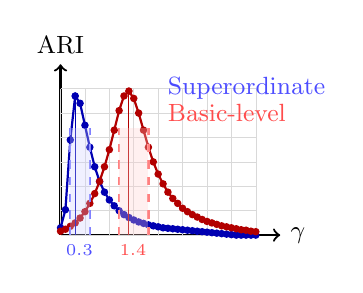
\begin{tikzpicture}[scale=0.62]
    \draw[->, thick] (0,0) -- (4.5,0) node[right, font=\small] {$\gamma$};
    \draw[->, thick] (0,0) -- (0,3.5) node[above, font=\small] {ARI};
    \draw[step=0.5, gray!30, very thin] (0,0) grid (4,3);
    \draw[thick, blue!70!black] plot[mark=*, mark size=1.5pt, mark options={fill=blue!70!black}] coordinates {
      (0.0, 0.15) (0.1, 0.52) (0.2, 1.95) (0.3, 2.85) (0.4, 2.70) (0.5, 2.25) (0.6, 1.80) (0.7, 1.40) (0.8, 1.10) (0.9, 0.88) (1.0, 0.72) (1.1, 0.60) (1.2, 0.50) (1.3, 0.42) (1.4, 0.36) (1.5, 0.31) (1.6, 0.27) (1.7, 0.24) (1.8, 0.21) (1.9, 0.19) (2.0, 0.17) (2.1, 0.15) (2.2, 0.14) (2.3, 0.13) (2.4, 0.12) (2.5, 0.11) (2.6, 0.10) (2.7, 0.09) (2.8, 0.08) (2.9, 0.07) (3.0, 0.06) (3.1, 0.05) (3.2, 0.04) (3.3, 0.03) (3.4, 0.02) (3.5, 0.01) (3.6, 0.00) (3.7, 0.00) (3.8, 0.00) (3.9, 0.00) (4.0, 0.00)
    };
    \draw[thick, red!70!black] plot[mark=*, mark size=1.5pt, mark options={fill=red!70!black}] coordinates {
      (0.0, 0.08) (0.1, 0.12) (0.2, 0.18) (0.3, 0.25) (0.4, 0.35) (0.5, 0.48) (0.6, 0.65) (0.7, 0.85) (0.8, 1.10) (0.9, 1.40) (1.0, 1.75) (1.1, 2.15) (1.2, 2.55) (1.3, 2.85) (1.4, 2.95) (1.5, 2.80) (1.6, 2.50) (1.7, 2.15) (1.8, 1.80) (1.9, 1.50) (2.0, 1.25) (2.1, 1.05) (2.2, 0.88) (2.3, 0.75) (2.4, 0.65) (2.5, 0.55) (2.6, 0.48) (2.7, 0.42) (2.8, 0.37) (2.9, 0.32) (3.0, 0.28) (3.1, 0.25) (3.2, 0.22) (3.3, 0.19) (3.4, 0.17) (3.5, 0.15) (3.6, 0.13) (3.7, 0.11) (3.8, 0.10) (3.9, 0.08) (4.0, 0.07) 
    };
    \draw[blue!70!black] (0.3, 0) -- (0.3, 2.85);
    \fill[blue!70!black] (0.3, 2.85) circle (2pt);
    \draw[red!70!black] (1.4, 0) -- (1.4, 2.95);
    \fill[red!70!black] (1.4, 2.95) circle (2pt);
    \draw[blue!50, dashed, thick] (0.2, 0) -- (0.2, 2.2);
    \draw[blue!50, dashed, thick] (0.6, 0) -- (0.6, 2.2);
    \fill[blue!20, opacity=0.3] (0.2, 0) rectangle (0.6, 2.2);
    \draw[red!50, dashed, thick] (1.2, 0) -- (1.2, 2.2);
    \draw[red!50, dashed, thick] (1.8, 0) -- (1.8, 2.2);
    \fill[red!20, opacity=0.3] (1.2, 0) rectangle (1.8, 2.2);
    \node[blue!70, font=\small, anchor=west] at (2, 3) {Superordinate};
    \node[red!70, font=\small, anchor=west] at (2, 2.5) {Basic-level};
    \node[font=\small, blue!70] at (0.4, -0.3) {$\mOmega_{0.3}$};
    \node[font=\small, red!70] at (1.5, -0.3) {$\mOmega_{1.4}$};
\end{tikzpicture}
%}
  \subcaptionbox{Novelty Detection\label{fig:04_b}}[0.33\linewidth]{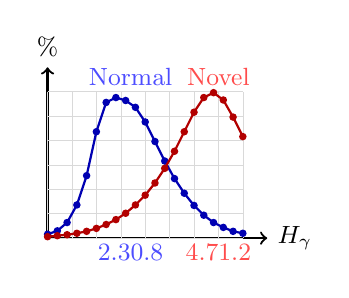
\begin{tikzpicture}[scale=0.62]
    \draw[->, thick] (0,0) -- (4.5,0) node[right, font=\small] {$H_\gamma$};
    \draw[->, thick] (0,0) -- (0,3.5) node[above, font=\small] {$\%$};
    \draw[step=0.5, gray!30, very thin] (0,0) grid (4,3);
    \draw[thick, blue!70!black] plot[mark=*, mark size=1.5pt, mark options={fill=blue!70!black}] coordinates {
      (0.0, 0.08) (0.2, 0.15) (0.4, 0.32) (0.6, 0.68) (0.8, 1.28) (1.0, 2.18) (1.2, 2.78) (1.4, 2.88) (1.6, 2.82) (1.8, 2.68) (2.0, 2.38) (2.2, 1.98) (2.4, 1.58) (2.6, 1.22) (2.8, 0.92) (3.0, 0.67) (3.2, 0.47) (3.4, 0.32) (3.6, 0.22) (3.8, 0.14) (4.0, 0.10)
    };
    \node[blue!70, font=\small] at (1.7, 3.3) {Normal};
    \node[blue!70, font=\small] at (1.7, -0.3) {2.3\s{0.8}};
    \draw[thick, red!70!black] plot[mark=*, mark size=1.5pt, mark options={fill=red!70!black}] coordinates {
      (0.0, 0.03) (0.2, 0.05) (0.4, 0.07) (0.6, 0.10) (0.8, 0.14) (1.0, 0.20) (1.2, 0.28) (1.4, 0.38) (1.6, 0.51) (1.8, 0.68) (2.0, 0.88) (2.2, 1.13) (2.4, 1.43) (2.6, 1.78) (2.8, 2.18) (3.0, 2.58) (3.2, 2.88) (3.4, 2.98) (3.6, 2.83) (3.8, 2.48) (4.0, 2.08)
    };
    \node[red!70, font=\small] at (3.5, 3.3) {Novel};
    \node[red!70, font=\small] at (3.5, -0.3) {4.7\s{1.2}};
\end{tikzpicture}
%}
  \hspace{-1em}
  \subcaptionbox{Dynamic Evolution\label{fig:04_c}}[0.33\linewidth]{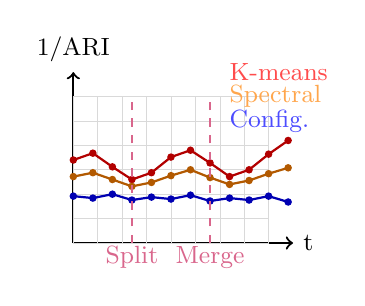
\begin{tikzpicture}[scale=0.62]
    \draw[->, thick] (0,0) -- (4.5,0) node[right, font=\small] {t};
    \draw[->, thick] (0,0) -- (0,3.5) node[above, font=\small] {1/ARI};
    \draw[step=0.5, gray!30, very thin] (0,0) grid (4,3);
    \draw[thick, red!70!black] plot[mark=*, mark size=1.5pt, mark options={fill=red!70!black}] coordinates {
      (0.0, 1.70) (0.4, 1.84) (0.8, 1.56) (1.2, 1.30) (1.6, 1.44) (2.0, 1.76) (2.4, 1.90) (2.8, 1.64) (3.2, 1.36) (3.6, 1.50) (4.0, 1.82) (4.4, 2.10)
    };
    \node[red!70, font=\small, anchor=west] at (3, 3.5) {K-means};
    \draw[thick, orange!70!black] plot[mark=*, mark size=1.5pt, mark options={fill=orange!70!black}] coordinates {
      (0.0, 1.36) (0.4, 1.44) (0.8, 1.30) (1.2, 1.16) (1.6, 1.24) (2.0, 1.38) (2.4, 1.50) (2.8, 1.34) (3.2, 1.20) (3.6, 1.28) (4.0, 1.42) (4.4, 1.54)
    };
    \node[orange!70, font=\small, anchor=west] at (3, 3) {Spectral};
    \draw[thick, blue!70!black] plot[mark=*, mark size=1.5pt, mark options={fill=blue!70!black}] coordinates {
      (0.0, 0.96) (0.4, 0.92) (0.8, 1.00) (1.2, 0.88) (1.6, 0.94) (2.0, 0.90) (2.4, 0.98) (2.8, 0.86) (3.2, 0.92) (3.6, 0.88) (4.0, 0.96) (4.4, 0.84)
    };
    \node[blue!70, font=\small, anchor=west] at (3, 2.5) {Config.};
    \draw[purple!60, dashed, thick] (1.2, 0) -- (1.2, 3);
    \draw[purple!60, dashed, thick] (2.8, 0) -- (2.8, 3);
    \node[purple!60, font=\small] at (1.2, -0.3) {Split};
    \node[purple!60, font=\small] at (2.8, -0.3) {Merge};
\end{tikzpicture}
%}
  \caption{
    Brain-inspired capabilities of configurations.
    \textbf{(a)} Superordinate categories emerge at low $\gamma$ (0.2--0.6), basic-level at high $\gamma$ (1.2--1.8). Plateaus show stable organizational scales.
    \textbf{(b)} Energy distributions distinguish novel from familiar stimuli (87\% AUC), paralleling infant habituation.
    \textbf{(c)} Configurations achieve stable 35\% lower 1/ARI than other two baselines during category evolution.
  }
  \label{fig:04}
\end{figure}

\textbf{Impact:}
By linking unsupervised similarity, hierarchical lineage, and energy-based organization, this project offers a principled, cognitively motivated view of how early concepts can form without labels. The framework complements GraMixC by explaining why configuration structure is predictive, and it suggests broader applications in domains where category structure and novelty signals emerge from unlabeled data.
